\documentclass[12pt,a4paper, twoside, pdftex, cleardoubleempty, pointlessnumbers]{scrbook}
% 12pt = Grundschrift, Papiergröße, beidseitiger Druck,
% cleardoubleempty = leere Seite ohne Kopfzeile, pointlessnumbers =
% Nummerierung ohne Punkt am Schluss
% !TeX spellcheck = de_DE
%-----------------------------------------------------------
%-------------------------- Pakete -------------------------

\usepackage[bottom=30mm, top=30mm, inner=35mm, outer=30mm]{geometry}	%legt Geometrie fest
\usepackage{ngerman}	%deutsche Rechtschreibung
%\usepackage[applemac]{inputenc}	%Umlaute für Mac
%\usepackage[latin1]{inputenc}		%Umlaute für Win
\usepackage[utf8]{inputenc}		%Umlaute für Linux
\usepackage{amsmath}			%Zusatzpaket für Formellayout
\usepackage[version=3]{mhchem}		%für chemische Formeln
\usepackage[small,hang]{subfigure}	%erlaubt nummerieren von Bilder, hang=hängender Einzug, small=Schriftgröße
\usepackage{graphicx}			%Einbinden von Bildern
\usepackage{subfigure}			%erweiterte Darstellungsoptionen für Bilder
\usepackage[usenames]{color}		%farbiger Text
\usepackage[labelfont=bf,textfont=normalsize]{caption}
\renewcommand{\figurename}{Abb. }	%ändert Abbildung in Abb.
\usepackage{hyperref}			%Inhaltsverzeichnis verlinkt
\usepackage{textcomp}
\usepackage{amssymb}
\usepackage{verbatim} 			%für "Computerschrift"
\usepackage{url}			%für Websites
\usepackage{parskip}			%Leerzeile statt Einrückung nach einem Absatz
\usepackage{epstopdf}
%\usepackage{natbib}
\addtokomafont{sectioning}{\rmfamily}	%ändert die serifenlose Überschrift in Roman

%-----------------------------------------------------------
%---------- Einstellungen für Kopf- und Fußzeile -----------

\setlength{\headheight}{15pt}
\usepackage{fancyhdr}			% Paket für Kopf- und Fußzeile  -  umfangreicher als "scrpage2"
\pagestyle{fancy}
\renewcommand{\headrulewidth}{.5pt}
\renewcommand{\footrulewidth}{0pt}
\renewcommand{\sectionmark}[1]{\markright{\textsl{\thesection \ #1}}}
\renewcommand{\chaptermark}[1]{\markboth{\thechapter \ #1}{}}
\fancyhf{} 					%löscht Kopf- und Fußzeile 
\fancyhead[LE,RO]{\thepage}			%\fancyhead[LE,RO]{\bfseries \thepage}
\fancyhead[RE]{\slshape\leftmark}
\fancyhead[LO]{\slshape\rightmark}

%-----------------------------------------------------------
%----------- für Kapitelanfänge etc. leere Seite -----------

\fancypagestyle{plain}{
		\fancyhead[LE,RO]{\thepage}
		\fancyhead[RE]{\slshape\leftmark}
		\fancyhead[LO]{\slshape\rightmark}
		\fancyfoot{}
		\renewcommand{\headrulewidth}{0.5pt}
		\renewcommand{\footrulewidth}{0pt}
}

%-----------------------------------------------------------

\graphicspath{{Grafiken/}}	
\DeclareGraphicsExtensions{.png}
\DeclareGraphicsExtensions{.eps}

%-----------------------------------------------------------

\setlength{\parindent}{0pt}			% Einrücken bei einem Absatz, 0pt => kein Einrücken

%----------------------------------------------------------
%Trennungsausnahmen (nicht für deutsche Umlaute)
\hyphenation{Alu-minium}
\hyphenation{Gleit-ebenen}

%----------------------------------------------------------
%Neue Befehle definieren

\newcommand{\abb}[1]{(Abb.~\ref{#1})} 		%Abbildungsreferenz: (Abb. <Nr>)
\newcommand{\abbohne}[1]{Abb.~\ref{#1}} 	%Abbildungsreferenz ohne Klammern: Abb. <Nr>
\newcommand{\kap}[1]{Kap.~\ref{#1}}		%Kapitelreferenz: Kap. <Nr>
\newcommand{\kapmit}[1]{(Kap.~\ref{#1})}	%Kapitelreferenz mit Klammern: (Kap. <Nr>)
\newcommand{\tabelle}[1]{Tabelle~\ref{#1}}	%Referenzierung einer Tabelle: Tabelle <Nr>
\newcommand{\Gl}[1]{Gl.~(\ref{#1})}		%Referenzierung einer Gleichung: Gl. (<Nr>)
\newcommand{\Gln}[1]{Gln.~(\ref{#1})}		% für mehrere Gleichungen mit einer gemeinsamen Nummer

% zwei mögliche Definitionen des "entspricht"-Zeichens
\newcommand{\entspricht}{\mathrel{\widehat{=}}}
\newcommand{\entsprichtapprox}{\mathrel{\widehat{\approx}}}

%-----------------------------------------------------------
%------------------------- Dateien -------------------------

\begin{document}


\frontmatter


		\setcounter{secnumdepth}{3}		% Numerierung bis subsubsection wird dadurch festgelegt
		\setcounter{tocdepth}{3}		% Gliederung subsubsection wird in Inhaltsverzeichnis eingetragen

		\thispagestyle{empty}

\begin{figure}[h]
\centering
\begin{minipage}{0.4\textwidth}
\subfigure{
\includegraphics[height=4cm]{Logo_HKA_IWI_Wortmarke_RGB.jpg}}\hfill
\end{minipage}
\hfill
\begin{minipage}{0.55\textwidth}
\hfill
\subfigure{ 
\includegraphics[height=4.0cm]{Logo_HKA_IWI_Bildmarke-h_RGB.jpg}}
\end{minipage}
\end{figure}

\begin{center}
\sffamily
%Hochschule Karlsruhe - University of Applied Sciences \\
%Fakultät für Informatik und Wirtschaftsinformatik\\
%Fachgebiet Wirtschaftsinformatik

\vspace{2.5cm}

\huge
\textbf{MASTERTHESIS}  % oder Bachelorarbeit
\vspace*{1cm}

\large
\textbf{Titel}  % kann über mehrere Zeilen gehen (Abstände ggf anpassen)

\vspace*{2.8cm}

\normalsize
\end{center}

\begin{tabular}{ll}
Autor: & Nico Kälble \\
Matrikelnummer: & 60791 \\
Arbeitsplatz: & SoftProject GmbH\\
Erstbetreuer: & Prof. Dr.-Ing. Jan Stoess\\
Zweitbetreuerin: & Prof. Dr. Rainer Neumann\\
Firmenbetreuer: & Patrick Toball\\
Tag der Abgabe:& 1.10.2024\\
\end{tabular}
\vspace{2cm} 



\normalsize

\clearpage

%%%%%%%%%%%%%%%%%%%%%%%%%%%%%%%%%%%%%%%%%%

% leere Seite
% \newpage
% \thispagestyle{empty}
% \vspace*{1cm} 
\raggedbottom
\cleardoublepage

		\clearpage
		\thispagestyle{empty}
\setcounter{page}{3}       % anpassen: wenn 1 Seitig  dannn 2     
%\pagestyle{scrheadings}

\chapter*{}
\centerline{\Large \textsf{\textbf{Erklärung}}} \label{Erklaerung}%\\
\vspace*{2ex}
%
Ich erkläre an Eides statt, dass ich die hier vorgelegte Masterthesis
selbstständig und ausschließlich unter Verwendung der angegebenen
Literatur und sonstigen Hilfsmittel verfasst habe. Die Arbeit wurde in
gleicher oder ähnlicher Form keiner anderen Prüfungsbehörde zur
Erlangung eines akademischen Grades vorgelegt.\\

\vspace{1.5cm}

Karlsruhe, 01.01.2021 \hfill
$\ldots \ldots \ldots \ldots \ldots \ldots \ldots \ldots \ldots \ldots \ldots \ldots$\

\hspace*{10cm} Nico Kälble


\vspace{4cm}

%------------Sperrvermerk (nur falls von Firma gewünscht) --------

\section*{}
\centerline{\Large \textsf{\textbf{S p e r r v e r m e r k}}} %\\

Diese Arbeit enthält vertrauliche (oder:  geheime) Informationen. 
Veröffentlichungen insbesondere vor dem (*31.12.2021) 
bedürfen der schriftlichen Genehmigung der (Organisation).

%%**************************************************************

\raggedbottom
\cleardoublepage

		\clearpage
		\section*{Kurzfassung der Arbeit} \label{Kurzfassung}
%
Die Kurzfassung gibt Auskunft über
\begin{itemize}
\item die Aufgabenstellung und Zielsetzung der Arbeit,
\item den technischen Zusammenhang, aus dem die Aufgabenstellung abgeleitet ist und
\item die wesentlichen Ergebnisse der Arbeit.
\item Die Kurzfassung ersetzt nicht die Zusammenfassung.
\end{itemize}



	
%\end{quotation}

\vspace{4cm}

\section*{Abstract} \label{Abstract}


Summary of the thesis in english language, maximum one page\\


\cleardoublepage
		\clearpage

		\addtocontents{toc}{}  			% Inhaltsverzeichnis (wird automatisch aus den Chapters und Section erstellt)
%		\addtocontents{toc}{\protect\thispagestyle{empty}} 		% Keine Kopf-/Fußzeile bei Inhaltsverzeichnis
		\tableofcontents			% Inhaltsverzeichnis

		\newpage				% nötig um korrekte Seitenzahlen bei mehrseitigem Inhalts-/Abb.verzeichnis
%		\pagenumbering{Roman}			% römische Seitenzahl für Abbildungsverzeichnis
%		\setcounter{page}{1}			% Seitenzahlen werden ab Abbildungsverzeichnis durchnummeriert
		\listoffigures				% Abbildungsverzeichnis

\mainmatter

		\chapter{Einleitung}
\label{Einleitung}
Die Skalierung von Software, die auf relationalen Datenbank Management Systemen (RDBMS) basiert, erweist sich in der Praxis als anspruchsvoll. ACID-Eigenschaften (Atomicity, Consistency, Isolation, Durability) dieser Systeme gewährleisten zwar eine hohe Zuverlässigkeit und Datenintegrität, allerdings führen sie auch zu einer Einschränkung der horizontalen Skalierung. \cite{reis2023} Daher erweisen sich diese Systeme bei der Verarbeitung und Analyse von großen Datenmengen (Big Data) in Echtzeit nicht als ausreichend und es sind alternative Lösungsansätze zu evaluieren, um die erhöhten Anforderungen an die Skalierung zu erfüllen.

Die Verarbeitung und Analyse von Big Data ist zwar kein neues Forschungsfeld und es existieren bereits zahlreiche Lösungen und Ansätze in der Literatur. Allerdings ist die Auswahl einer geeigneten Technologie für spezifische Anwendungsfälle keineswegs trivial. Eine sorgfältige Evaluierung ist notwendig, da jede Technologie unterschiedliche Vor- und Nachteile bietet und die Entscheidung von vielen Faktoren abhängt, darunter die spezifischen Anforderungen der Anwendung, die vorhandene Infrastruktur und die gewünschten Performance-Eigenschaften. Die Auswahl der geeigneten Technologien und Architekturen erfordert daher eine gründliche Analyse und Abwägung, um sicherzustellen, dass die Lösung gegenwärtigen und zukünftigen Anforderungen an Flexibilität und Skalierung gerecht wird.

 Die vorliegende Masterarbeit widmet sich dieser Problematik am Beispiel der X4 Business Process Management Software (X4 BPMS), einer Software für die Geschäftsprozessautomatisierung. Ein besonderer Fokus liegt dabei auf den Aspekten der Modularität und Flexibilität bei der Integration in heterogene Systemlandschaften, die sich aus dem Einsatz der Software in unterschiedlichen Branchen und Projekten ergeben. 

\section{Motivation}
Die Motivation dieser Masterarbeit besteht darin, eine flexiblere und skalierbarere Datenmanagementlösung für die X4 Business Process Management Software (X4 BPMS) zu entwickeln, da die derzeitige Implementierung Leistungsprobleme beim Loggen und Analysieren großer Prozessdatenvolumen aufweist. Daher ist das Ziel dieser Arbeit, die aktuelle Implementierung in diesem Bereich zu untersuchen, Probleme herauszuarbeiten, Lösungsmöglichkeiten zu identifizieren und zu vergleichen sowie eine Lösung auszuwählen und durch eine prototypische Implementierung zu evaluieren. Die Lösung soll zum einen Prozessdaten der X4 BPMS auf skalierbare Art und Weise für heterogene Systemlandschaften bereitstellen können, sofern der Kunde die Daten in eigene BI- und Analyse-Lösungen integrieren möchte. Zum anderen soll sie eine skalierbare Standardlösung für Kunden bieten, welche Anforderungen an modernere, datenintensive Anwendungen erfüllt.

\section{Problem Statement}
Insbesondere im Hinblick auf die Skalierbarkeit sind Daten von Relevanz, die sich durch eine hohe Erzeugungsfrequenz sowie ein hohes Datenvolumen pro Zeiteinheit auszeichnen. Innerhalb der X4 BPMS sind dies primär Daten, die im Rahmen der Ausführung technischer Prozesse generiert werden, da diese wesentlich schneller Ablaufen als Prozesse, die menschliche Aktivitäten erfordern. Bei der Ausführung der modellierten Prozesse in der Process Engine der X4 BPMS werden für jeden Prozessschritt Events generiert, systematisch erfasst und gespeichert. Je nach Konfiguration erfolgt dieses Loggen entweder in Textform in das Dateisystem oder in Eventtabellen in ein RDBMS. In der Regel besteht neben der reinen Archivierung dieser Events auch das Interesse diese Eventdaten zu analysieren. Um dies zu ermöglichen wurde eine Web-Applikation entwickelt, die Anwendern eine nutzerfreundliche Oberfläche bereitstellt, ihre ausgeführten Geschäftsprozesse zu überwachen und zu analysieren. Diese Analyse- und Überwachungslösung wird als "Process Monitor" bezeichnet und wird Kunden der SoftProject GmbH kostenlos zur Verfügung gestellt.\cite{softprojectgmbh-ProcessMonitor-Webseite}
In Abbildung \ref{fig:Problemstellung} sind die Kernprobleme der aktuellen Implementierung des Process Monitors dargestellt, welche in Kapitel \ref{Systemübersicht} genauer beschrieben werden.
\begin{figure}
    \centering
    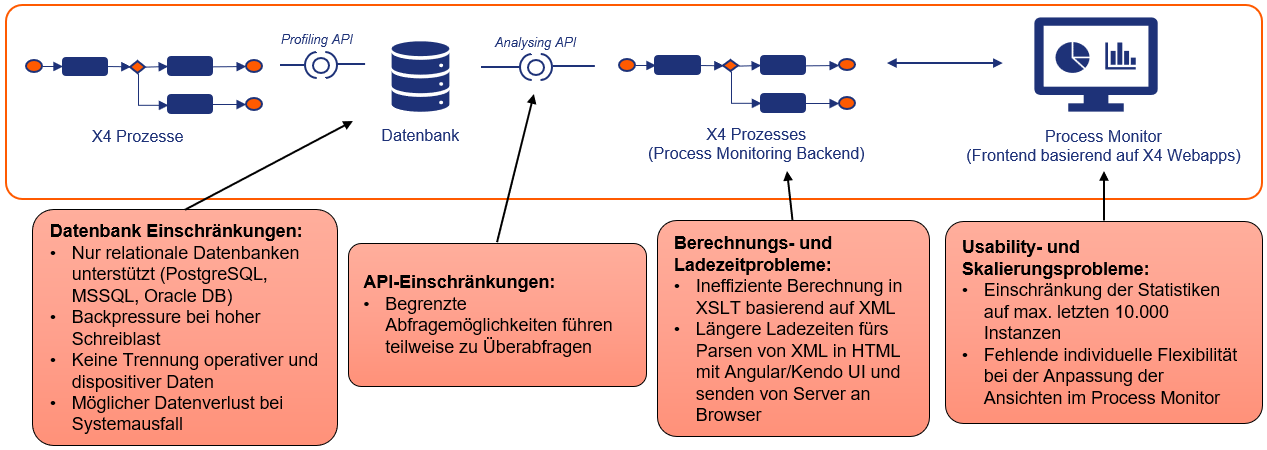
\includegraphics[width=1\linewidth]{Grafiken/Problemstellung.png}
    \caption{Darstellung der aktuellen Probleme}
    \label{fig:Problemstellung}
\end{figure}

Dabei birgt jede Phase im Datenmanagementprozess – von der Datenintegration, über Transformation und Speicherung bis hin zur Datenanalyse und Visualisierung – weitere spezifischere Herausforderungen und interdisziplinäre Fragestellungen mit sich. Diese Herausforderungen betreffen technische Aspekte wie Skalierbarkeit, Performance, Flexibilität und Integration sowie wirtschaftliche Faktoren wie Implementierungskosten, Time-to-Market, oder Kosten-Nutzen-Vergleich der Technologien.

Die Masterarbeit verfolgt das Ziel, diese komplexen Fragestellungen effizient auf ein reales Anwendungsszenario zu übertragen. Dabei wird untersucht, wie verschiedene disziplinäre Ansätze der Wirtschaftsinformatik – einschließlich Use-Case- und Systemanalyse, Technologieauswahl, Implementierung und Performanceoptimierung – kombiniert werden können, um eine effektive und skalierbare Datenmanagementlösung für die X4 BPMS zu entwickeln.

\section{Stand der Forschung}

Die vorliegende Arbeit widmet sich interdisziplinären Fragestellungen im übergeordneten Gebiet des Data Engineering, wobei der Fokus auf dem spezifischeren Kontext der Echtzeit Geschäftsprozessüberwachung mit großen Datenvolumina liegt. Es gibt bereits dedizierte Forschungsarbeiten die relevante Teilgebiete der Arbeit im Detail betrachten und Übersichtswerke die generelle Trends und Praktiken in beleuchten. Des weiteren gibt es Anbieter von Geschäftsprozessautomatisierungssoftware wie Camunda, Appian, Flowable, Mendix oder OutSystems, die im gleichen Branchenumfeld wie die SoftProject GmbH Lösungen für die Prozessüberwachung anbieten, wodurch dieser Forschungsbetrag diese in speziellen Kontext der X4 BPMS auf ihre Machbarkeit und Nutzen analysiert. 

\cite{CamundaOperate}

Beispielsweise behandeln Joe Reis und Matt Hously in einem Grundlagenwerk zum Thema Data Engineering grundsätzlich relevante Phasen, Aspekte und Fragestellungen anhand des "Data Engineering Lifecycles" von der Datengenerierung über Ingestion, Transformation, Speicherung und Bereistellung bis hin zur Analyse. \cite{reis2023} 

\section{Ansatz}

\section{Aufbau der Arbeit}
Im folgenden Kapitel \ref{StandDerForschung} werden Grundlagen
dargelegt und der Stand der Forschung diskutiert. In Kapitel
\ref{Ansatz} wird der Ansatz genauer beleuchtet. Im Kapitel
\ref{Implementierung} wird die Umsetzung des Ansatzes
beschrieben. Kapitel \ref{Validierung} praesentiert Resultate und eine
Diskussion der Ergebnisse. Im Kapitel \ref{ZusammenfassungAusblick}
wird die Arbeit zusammengefasst, ein Fazit gezogen und ein Ausblick
auf zukuenftige Arbeiten gegeben.

 

		\chapter{Grundlagen und theoretischer Rahmen}
\label{StandDerForschung}

\section{Datenintegration und -analyse}
Relevante Quellen:
\begin{itemize}
    \item IT-Management\cite{tiemeyer2023}
    \item Data Engineering \cite{reis2023}
    \item BPM Übersicht \cite{weske2019}
    \item 
    \item Speziellere Werke zum Thema
\end{itemize}


Joe Reis und Matt Hously gehen in einem Grundlagenwerk zum Thema Data Engineering auf grundsätzlich relevante Phasen, Aspekte und Fragestellungen anhand des "Data Engineering Lifecycles" von der Datengenerierung über Ingestion, Transformation, Speicherung und Bereistellung bis hin zur Analyse ein. \cite{reis2023} 


\begin{itemize}
\item Hier wird auf Literatur im Bereich Datenintegration und Analyse eingegangen
\item Das Kapitel gibt einen groben Überblick welche Aspekte basierend auf Literatur im Bereich Datenintegration und Analyse beachtet werden müssen
\item Wichtigstes Grundlagenwerk ist das „Handbuch Data Engineering: Robuste Datensysteme planen und erstellen“ von Joe Reis und Matt Housley, welches das Forschungsgebiet "Data Engineering" umfassend beschreibt, Grundbegriffe definiert und relevante Konzepte behandelt und auf weitere relevante Quellen verweist.
\end{itemize}

Der wesentliche Teil der Arbeit lässt sich dem Themengebiet \textit{Data Engineering} zuordnen. Das wohl bekannteste Grundlagenwerk in diesem Themengebiet ist das Buch \textit{Fundamentals of Data Engineering: Plan and Build Robust Data Systems} von Joe Reis und Matt Housley, die unterschiedliche Definitionen des Begriffs \textit{Data Engineering} vorstellen und ihn zusammenfassend wie folgt definieren (in Deutsche übersetzt) \cite{reis2023}:

\begin{quote}
    \textit{Data Engineering ist die Entwicklung, Implementierung und Wartung von Systemen und Prozessen, die Rohdaten aufnehmen und hochwertige, konsistente Informationen erzeugen, die nachgelagerte Anwendungsfälle wie Analysen und Machine Learning unterstützen. Data Engineering ist die Schnittstelle zwischen Sicherheit, Datenmanagement, DataOps, Datenarchitektur, Orchestrierung und Softwareentwicklung.}
\end{quote}

Reis und Housley etablierten mit den \textit{Data Management Lifecycle} (siehe \autoref{fig:Data Engineering Lifecycle}) außerdem eine systematische, praxisorientierte und mittlerweile verbreitete Abgrenzung der Themenbereiche des \textit{Data Engineerings}. 

\begin{figure}
    \centering
    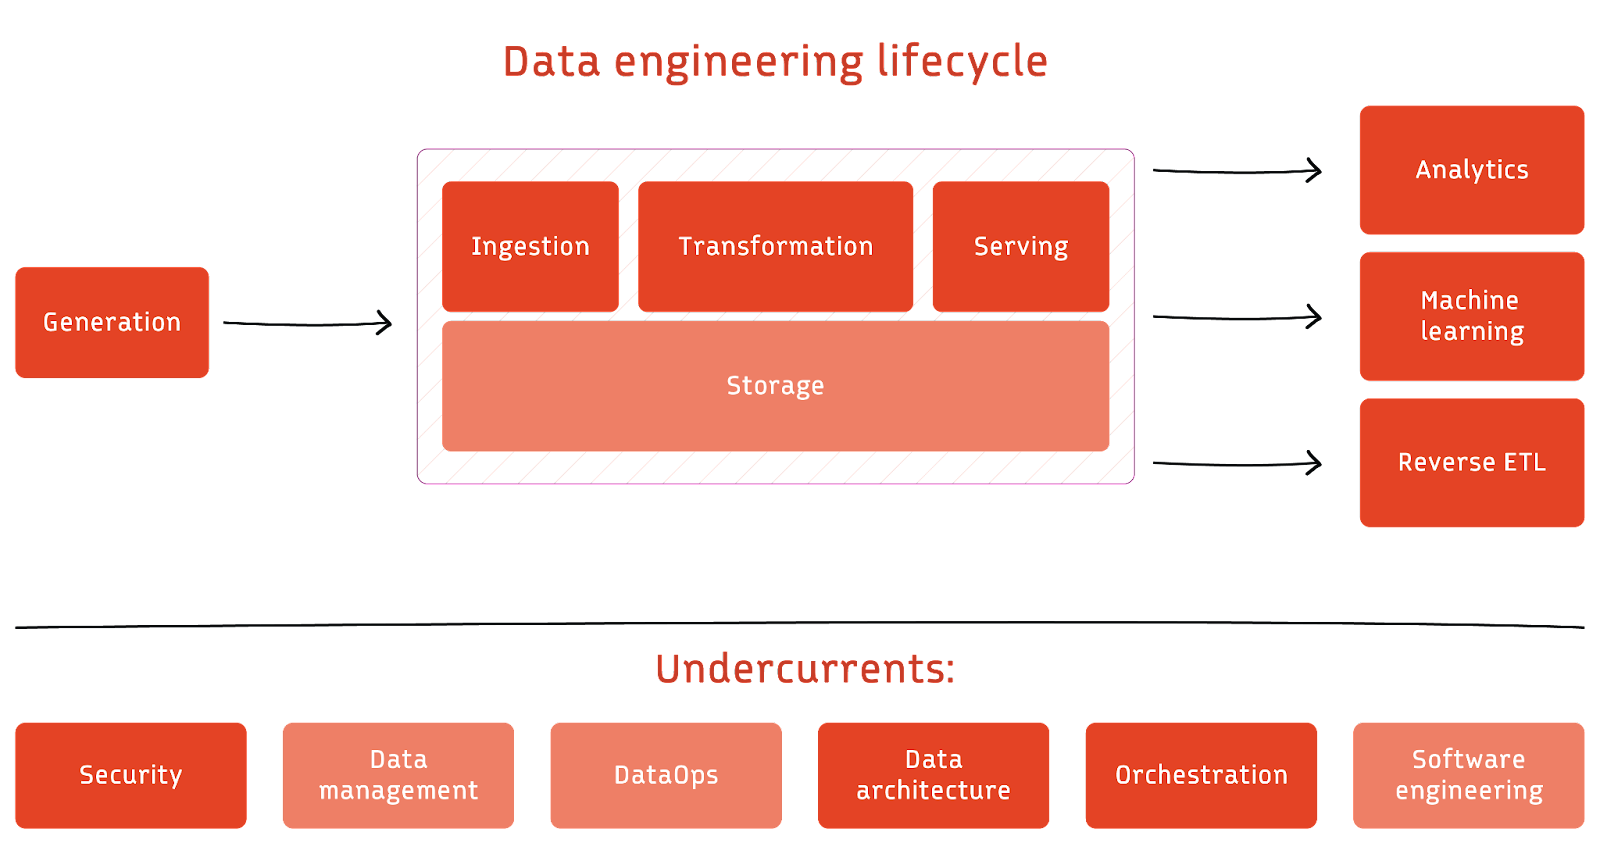
\includegraphics[width=1\linewidth]{Grafiken/Data Engineering Lifecycle.png}
    \caption{Data Engineering Lifecycle}
    \label{fig:Data Engineering Lifecycle}
\end{figure}

\subsection{Grundlagen zu Materialien}

\section{Systemübersicht - Die X4 BPMS und datengetriebene Geschäftsmodelle}
\label{Systemübersicht}

\subsection{Allgemeine Grundlagen der X4 BPMS}
\subsection{Daten und Schnittstellen der X4 BPMS}
\subsection{Analyse der Anwendungsfälle und Anforderungen an die X4 BPMS}

\section{Bestehende Ansätze und Technologien}
\subsection{Allgemeine Konzepte und Technologien}
OLAP vs. OLTP \cite{kleppmann2017} S. 91 in "Designing Data Intensive Applications" 

\subsection{Vorstellung existierenderLösungen und Produkte im Kontext der Geschäftsprozessüberwachung}
\subsection{Zusammenfassung der Ergebnisse}


		\chapter{Ansatz}
\label{Ansatz}


\section{Technologieevaluation}

\section{Vorstellung der Lösungsarchitektur}



		\chapter{Implementierung}
\label{Implementierung}

In der Konzeption wurden alle relevanten Entscheidungen getroffen, so
dass es in diesem Kapitel typischerweise nur noch um technische
Aspekte und Implementierungsdetails geht. Im Idealfall enthält dieses
Kapitel also keine ``Überraschungen'' auf konzeptioneller Ebene,
sondern beschreibt lediglich Besonderheiten der Implementierung, die
etwa jemand, der das System nachbauen oder nachvollziehen möchte,
wissen sollte. Zu beachten ist dabei, dass die Implementierung
grundsätzlich nur ein Mittel zur Beantwortung und Validierung der
Frage ist, und kein Selbstzweck. Sie dient – zumindest was die
Bearbeitung der Thesis betrifft – nur einem einzigen Ziel: der
Validierung (Kapitel \ref{Validierung}), ob der vorgestellte Entwurf
(Kapitel \ref{Ansatz}) die Problemstellung (Kapitel \ref{Einleitung}
tatsächlich erreicht.

Es kann (muss aber nicht zwingend) sinnvoll sein, das Kapitel
Implementierung analog zur Konzeption zu strukturieren. Hat man zum
Beispiel verschiedene Teile eines Gesamtsystems entworfen (in Kapitel
\ref{Ansatz}), kann man die Implementierung dieser Teile in analoger
Struktur (Kapitel \ref{Implementierung}) vorstellen.

\section{Umsetzung meines Verfahrens 1}
\label{MeinsImplementierung1}

Verfahren 1 habe ich komplett implementiert, getestet und produktiv
gesetzt, es läuft seit 10 Jahren fehlerfrei und macht insbesondere
meine Chefin total gluecklich.

\section{Umsetzung meines Verfahrens 2}
\label{Meins2Implementierung}

Verfahren 2 habe ich gar nicht umgesetzt, es bleibt komplettes
Papierdesign, aber es funktioniert bestimmt.

		\chapter{Validierung}
\label{Validierung}
Hier werden Konzept und Implementierung in Hinblick auf die
Problemstellung validiert. Die eigentliche Validierung kann ganz
unterschiedlich erfolgen. Stehen quantitative Ziele im Vordergrund
(Performance, Latenz, Durchsatz, Skalierung, Kosten), kann die
Validierung aus Messungen und empirischen Untersuchungen
bestehen. Stehen technisch-funktionale Aspekte im Vordergrund (``ist
machbar''), kann die Validierung aus einer qualitativen Begutachtung
der eigenen Konzeption und Implementierung bestehen. Stehen soziale
oder ``menschliche'' Ziele im Raum, kann die Validierung Befragungen
oder Interviews enthalten. Kombinationen sind natürlich erlaubt.

Ziel ist eine gesamthafte, überzeugende und strukturierte Validierung
der eigenen Konzeption im Hinblick auf das Ziel. Ob das Ziel erreicht
wurde oder nicht, ist dabei im Grunde sekundär – auch negative
Resultate (``geht nicht'', ``ist zu langsam'') können sehr gute
Resultate sein. Wichtig ist das methodische Vorgehen zur Beantwortung
der Frage.

\section{Resultate}

\subsection{Das habe ich gemessen 1}
\label{Ergebnisse_1}

\subsubsection{Messungen unter Bedingung 1}

Hier stehen viele bunte Bilder. Also die Ergebnisse der Messungen/Rechnungen...

\subsubsection{Messungen unter Bedingung 2}

\subsection{Das habe ich berechnet 2}
\label{Ergebnisse_2}

\subsubsection{Rechenergebnisse mit Modell 1}

\subsubsection{Rechenergebnisse mit Modell 2}

\section{Interpretation}
\label{Interpretation}

Was bedeuten die ganzen Ergebnisse und was ist
das Fazit?\\ Während der Ergebnisteil neutral und objektiv die
Ergebnisse präsentieren soll, können hier verschiedene Ergebnisse
verglichen werden und Schlüsse gezogen werde sowie Bewertungen
abgegeben werden.

		\chapter{Zusammenfassung und Ausblick}
\label{ZusammenfassungAusblick}
Hier wird nochmal alles kurz zusammengefasst und gesagt, was nicht
gelöst werden konnte in der Kürze der Zeit.


\backmatter
		%\addtocontents{toc}{\newpage}
		%\addtocontents{toc}{\protect\thispagestyle{empty}}
		\appendix
		%---------------------------------------------------------- 
		\pagenumbering{Roman}					%Entfernt das "A" vor dem Anhang
		\setcounter{chapter}{1}	
		\renewcommand{\thechapter}{\Alph{chapter}}		%setzt alphabetische Numerierung

		\pagestyle{fancy}
		\renewcommand{\headrulewidth}{.5pt}
		\renewcommand{\footrulewidth}{0pt}
		\renewcommand{\sectionmark}[1]{\markright{\textsl{\thesection \ #1}}}
		\renewcommand{\chaptermark}[1]{\markboth{#1}{}}
		\fancyhf{} 	%löscht Kopf- und Fußzeile
		\fancyhead[LE,RO]{\thepage}
		\fancyhead[RE]{\slshape\leftmark}
		\fancyhead[LO]{\slshape\rightmark}
		%----------------------------------------------------------
		\chapter{Anhang}

\section{Ergänzende Diagramme}
\label{Anhang_Diagramme}

Hier könnte noch was stehen. Z.B. zusätzliche Diagramme, Gleichungen
oder erklärender Text, die für den Lesefluss im Haupttext hinterlich
sind, aber interessante zusätzliche Einblicke liefern.

\section{Ergänzende Codeschnipsel}
\label{Anhang_Code}

Hier könnten auch Code-Snippets stehen, die kein Mensch liest, die
aber ungeheueren Eindruck machen.

                \addcontentsline{toc}{chapter}{\bibname}%
		\bibliography{Literaturverzeichnis}{}
		\bibliographystyle{ThesisBibliographystyle}
\end{document}
